\documentclass[11pt]{article}

\usepackage{amssymb}
\usepackage{amsmath}
\usepackage{graphicx}
\usepackage{cite}
%\usepackage{algorithmic}
%\usepackage{algorithm}
\usepackage{todonotes}
\usepackage{url}
\usepackage{tikz}
\usetikzlibrary{arrows}

\usepackage{caption}
\usepackage{subcaption}


\usepackage{listings}
 \lstset{
            language=Matlab,                                % choose the language of the code
    %       basicstyle=10pt,                                % the size of the fonts that are used for the code
            numbers=left,                                   % where to put the line-numbers
            numberstyle=\footnotesize,                      % the size of the fonts that are used for the line-numbers
            stepnumber=1,                                           % the step between two line-numbers. If it's 1 each line will be numbered
            numbersep=5pt,                                  % how far the line-numbers are from the code
    %       backgroundcolor=\color{white},          % choose the background color. You must add \usepackage{color}
            showspaces=false,                               % show spaces adding particular underscores
            showstringspaces=false,                         % underline spaces within strings
            showtabs=false,                                         % show tabs within strings adding particular underscores
    %       frame=single,                                           % adds a frame around the code
    %       tabsize=2,                                              % sets default tabsize to 2 spaces
    %       captionpos=b,                                           % sets the caption-position to bottom
            breaklines=true,                                        % sets automatic line breaking
            breakatwhitespace=false,                        % sets if automatic breaks should only happen at whitespace
            escapeinside={\%*}{*)}                          % if you want to add a comment within your code
}

\setlength{\paperwidth}{8.5in}
\setlength{\paperheight}{11in}
\setlength{\voffset}{-0.2in}
\setlength{\topmargin}{0in}
\setlength{\headheight}{0in}
\setlength{\headsep}{0in}
\setlength{\footskip}{30pt}
\setlength{\textheight}{9.25in}
\setlength{\hoffset}{0in}
\setlength{\oddsidemargin}{0in}
\setlength{\textwidth}{6.5in}
\setlength{\parindent}{0in}
\setlength{\parskip}{9pt}

\newcommand{\ben}{\begin{enumerate}}
\newcommand{\een}{\end{enumerate}}

\DeclareGraphicsRule{.JPG}{eps}{*}{`jpeg2ps #1}

\title{Streaming Graph Partitioning \\ Progress Update}
\author{Casey Battaglino\\Robert Pienta}
\date{}
\begin{document}
\maketitle
\section*{Introduction} \vspace{-10 pt}
Our project investigates the process of partitioning a graph using a \emph{streaming} partitioner. Graph partitioning has been a part of theoretical computer science for decades, but saw increasing attention in the 1990s as a method of partitioning problems to increase parallel locality. 

The balanced graph partitioning problem can be stated as such: we wish to partition the nodes of a graph into $k$ components with capacity $(1+\epsilon)\frac{N}{k}$, such that cost is minimized, where cost is generally the number of edges that cross partition boundaries. Requiring both balance and cost-minimization places this problem in NP-complete, because it becomes a minimum-bisection problem~\cite{Garey:1979:CIG:578533}.

Offline graph partitioning algorithms, where the graph is allowed to exist in memory, have existed for decades. Hundreds of variants of such algorithms likely now exist, and range from spatial methods to spectral methods~\cite{arora2009expander}. The most scalable and effective graph partitioners on massive datasets are currently multi-level partitioners, which contract the graph to a small number of vertices, and then heuristically optimize the problem on each subsequent expansion~\cite{karypis1998multilevel}. 

\section{Streaming Graph Partitioning}\vspace{-10 pt}
Streaming graph partitioning has only been introduced in the last couple of years~\cite{DBLP:journals/corr/abs-1212-1121,Stanton:2012:SGP:2339530.2339722,tsourakakis2012fennel}, as graphs grow to the point where they may not fit into memory, or must be distributed to compute nodes on the fly. In the streaming model, input data (vertices) arrive sequentially from a generating source (such as a web-crawler), and must be partitioned as they arrive. As an example, partitioning the Twitter graph can take nearly a day using the fastest offline algorithms, but can take a matter of minutes using a streaming algorithm.

\subsection{Streaming Heuristics}
Assuming vertices arrive in a stream (which may come in a BFS, DFS, random, or adversarial ordering), a heuristic makes a partition decision, given vertex $v$, and capacity constraint $C$ (where $C$ is generally $\approx \frac{(\epsilon+|V|)}{n}$ Stanton presents the following heuristics, roughly in order from most naive to most complex~\cite{Stanton:2012:SGP:2339530.2339722}: (only the un-buffered heuristics are presented)

\begin{enumerate}
\item Balanced: assign $v$ to partition of minimum size, with random tie breaking.
\item Chunking: divide input stream into chunks of size $C$.
\item Hashing: assign $v$ to $H(v)$, where $H$ is hash function $F:V\to\{1\dots k\}$
\item Weighted Deterministic Greedy (WDG): Assign $v$ to partition that it has most edges to, weighted by the relative size of each partition (weight function can be linear or exponential).
\item Weighted Randomized Greedy: Assign $v$ randomly according to a probability distribution defined by the weights of each partition in WDG.
\item Weighted Triangles: Assign $v$ to partition whose intersection with $v$ contains the most triangles, weighted by the relative size of each partition.
\item Balance Big: for high-degree $v$, use Balanced. For low-degree $v$, use WDG. 
\end{enumerate}

Of note is that many major graph-processing toolkits such as GraphLab~\cite{Low:2012:DGF:2212351.2212354} use the hashed (random) partitioning method, which essentially produces a worst-case edgecut of size $\frac{k-1}{k}|E|$, but which has the benefit that $H(v)$ can be called at any time to return the compute node that owns $v$. 

In Stanton's experimental results~\cite{Stanton:2012:SGP:2339530.2339722}, WDG performed far better than any other partitioner. FENNEL~\cite{tsourakakis2012fennel} is a heuristic that generalizes the WDG partitioner for any weight function, and provides a somewhat more rigorous theoretical framework. 


\section{Initial Steps}
Our first goal was to implement the partitioning methods developed in recent literature, and test them with on synthetic graphs. This paves the way for us to make further contributions to the field (given that we can now compare any techniques we come up with to the techniques in the literature).

Our `test-bed' is implemented in MATLAB, because many important properties of graphs can be easily extracted using vector notation on their adjacency matrices, and code is very easy to prototype. Our code located at~\url{https://github.com/cjbattagl/graphpart/tree/master/mfiles}

We measured the overall quality of partitions by the \textit{fraction of cut edges} $\lambda$.
\[\lambda = \frac{\text{Number of edges cut by partition}}{\text{Total number of edges}}\]

We investigated the results for the simplest case of partition, the bi-partition or 2-partition, but will continue our tests onto generic k-partitions.  
We have also performed an analysis of the parameters used by FENNEL.

\section*{Synthetic Tests} \vspace{-10 pt}
Our initial tests focus on the partitioner FENNEL which purports to have comparable performance in the quality of partitions with METIS, but with drastically faster computation time on large graphs. 

\begin{figure}[ht]
\centering
\caption{A sample adjacency matrix for a partitioned ER graph (n=1000, m=1962), $\gamma = 1.5$}
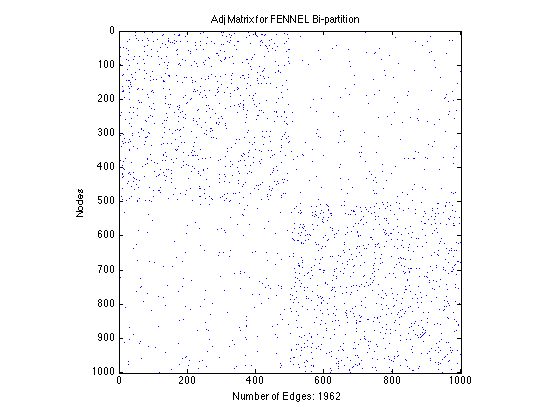
\includegraphics[scale=.65] {figures/adj_spy.png}
\label{fig:1}
\end{figure}

\subsection*{Experiments} \vspace{-10 pt}
We examined the quality of FENNEL partitions over ER graphs with 1000 nodes and variable numbers of edges. Each point is the average of multiple ER graph partitions. Figure~\ref{fig:1} shows an example partition that we produced on an Erdos-Renyi graph, and demonstrates how a spy plot can be used to eyeball the quality of a partition.

\begin{figure}[ht]
\caption{FENNEL experiments investigating partition quality versus graph density and parameter choice.} 
\begin{subfigure}[b]{0.5\textwidth}
\caption{Average $\lambda$ of partition compared against varied density ER graphs (n=1000).  FENNEL's performance quickly degrades as the random graph grows in edge-density.}
\label{figure:quality}
\centering
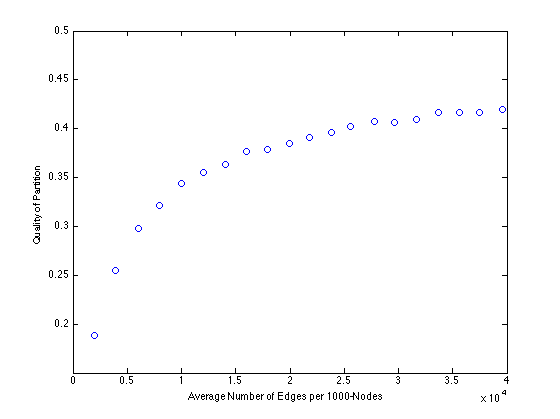
\includegraphics[width=\textwidth] {figures/varied_er_p.png}
\end{subfigure}
\begin{subfigure}[b]{0.5\textwidth}
\caption{Average $\lambda$ of partition compared against varied $\gamma$ for ER graph (n=1000, p=0.001)  The results on $(1,2)$ do not yield differences in performance on ER Graphs.}
\label{figure:gamma}
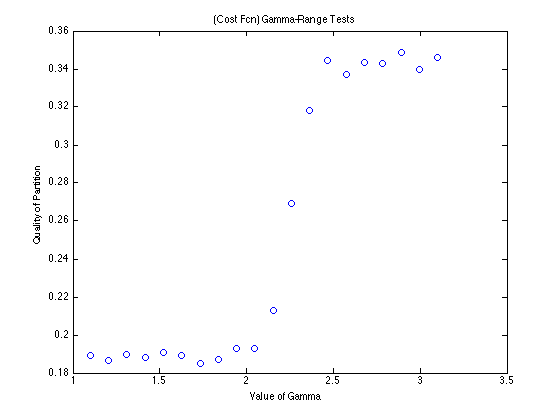
\includegraphics[width=\textwidth] {figures/varied_gamma.png}
\end{subfigure}
\end{figure}
FENNEL uses a deterministic greedy partitioner penalized via a cost function of the form $c(x) = \alpha x^\gamma$, where $x$ is the number of nodes in a partition. 
For $1\le\gamma\le 2$ the cost function balances between adding the new vertex to the partition with the largest number of neighbors and the least number of non-neighbors respectively.
Next we investigated the input parameters to the FENNEL costs function in Figure \ref{figure:quality}.  

Note that in Figure \ref{figure:gamma}, the increase in the cost function past a quadratic incurs a sharp loss in quality as it very heavily suggests the placement of vertices into partitions with the lowest number of non-neighbors.

We tested two suggestions for $\alpha$ with multiple runs on ER graphs.
The results shown in Table \ref{table:qualityalpha}
\begin{table}[ht]
\centering
\caption{The quality of partitions by choice of $\alpha$}
\label{table:qualityalpha}
\begin{tabular}{r | r}\hline
Graph & Ave $\lambda$ \\ \hline &\\
$\sqrt{2}\frac{m}{n^1.5}$ & 18.17\\ &\\
$\vspace{3pt}m\frac{2^\gamma-1}{n^\gamma} $&18.37\\
\end{tabular}
\end{table}



In order to test scale-free distributions we chose to use Kronecker generated scale free network with $n=8192, m=16384$. (Note: Table~\ref{table:quality} is just a small subset of what we plan to investigate).

\begin{table}[h]
\centering
\caption{The quality of partitions}
\label{table:quality}
\begin{tabular}{r | c}\hline
Graph & $\lambda$ \\ \hline
ER & \\
Kronecker Scale-Free & 30.80\\
others & etc..\\
\end{tabular}
\end{table}
\newpage
\section{Current Status}
We have currently implemented the basic heuristics (balanced, chunking, hashing), the greedy heuristics (deterministic/random greedy), and the generalized partitioner FENNEL. We have generators for E-R, hidden-partition, and Power-Law (RMAT/Kronecker) graphs, and we have also downloaded the entire SNAP real-world network data set and the Twitter graph. Thus, we have a test-bed upon which we can test any of our additional contributions. 

As our early experiments demonstrate, we are also able to investigate the quality of partitioners as the parameters of the random graphs change, which is not an experiment performed in the literature. This is of particular interest for Kronecker Power-Law graphs, which are seeded with 4 parameters (which can be fitted to real-world graphs using a \texttt{Kron-Fit}  package).

\section{Next Steps}
\begin{enumerate}
\item Propose new partitioning heuristics and evaluate them.
\item Investigate critical points of failure of heuristics on random graph models, and justify.
\item Evaluate heuristics with other objective functions (such as edge-partitioning).
\end{enumerate}


\section{Example MATLAB Code}
Here is an example of MATLAB code that we developed to perform a streaming heurisic (FENNEL) on an input graph. In this case, streaming order is a random permutation on $\{1\dots N\}$.
\begin{verbatim}
%Input: Adjacency Matrix A, Weight parameter gamma
%Output: Bisected adjacency matrix B = A(p,p)
function [B] = fennel (A, gamma)
  vorder = randperm(size(A,1));

  m = size(A,1);
  e = nnz(A);

  alpha = sqrt(2)*e/m^1.5;

  p1 = [];
  p2 = [];
  
  for v=vorder
    idxs = find(A(v,:));  %get N(v)

    [~, loc] = ismember(idxs, p1); %set loc to idxs of intersect(N(v), S1)
    loc = find(loc); %length(loc) is now number of edges between v, S1
    p1newedges = -length(idxs) + length(loc); %p1newedges is number of edges between v, V \ S1 = e(v, V \ S1)
    clear loc
    
    [~, loc] = ismember(idxs, p2);
    loc = find(loc);
    p2newedges = -length(idxs) + length(loc);

    % if h(S2) + h(S1 U {v}) > h(S1) + h(S2 U {v})
    if (p1newedges - dc(length(p1),alpha, gamma)) >= (p2newedges - dc(length(p2),alpha,gamma))
      p1 = [p1 v];
    else
      p2 = [p2 v];
    end
  end

  B = A([p1 p2],[p1 p2]); 
end

function [dy] = dc(x, alpha, gamma)
  dy = c(x+1, alpha, gamma) - c(x, alpha, gamma);
end
\end{verbatim}

\bibliographystyle{plain}
\bibliography{bib}


\end{document}